\chapter{Arhitektura i dizajn sustava}
		

		\textit{Arhitektura se sastoji od 3 podsustava:}
	\begin{itemize}
		\item 	\textit{Web poslužitelj}
		\item 	\textit{Web aplikacija}
		\item 	\textit{Baza podataka}		
	\end{itemize}
	
			Web poslužitelj omogućuje komunikaciju klijenta s aplikacijom, pomoću HTTP (Hyper Text Transfer Protocol) protokola. HTTP protokol je protokol aplikacijskog sloja koji služi za razmjenu svih podataka (HTML stranica, slika, itd.) na Internetu. Dvije glavne metode HTTP protokola su GET i POST metode. GET (HTTP GET) metoda se koristi kao zahtjev za podacima na serveru, a POST (HTTP POST) metoda se koristi za kreiranje ili ažuriranje podataka na serveru. Uspostava veze se odvija tako da se klijent spoji na port 80 i web poslužitelju uputi zahtjev za traženom stranicom, a on mu vraća HTML kod tj. HTML stranicu ili ju izgenerira. Web poslužitelj zapravo pokreće aplikaciju te joj proslijeđuje zahtjev. Klijent prima HTML kod te ga prikazuje u obliku stranice. Sam korisnik upućuje zahtjev preko web preglednika. Web aplikacija služi za obrađivanje željenih zahtjeva. Kroz HTTP zahtjeve ćemo dohvaćati podatke u formatu JSON, a u web aplikaciji ih obrađivati te preslikavati u bazu podataka. Bazu podataka ćemo napravili u PostgreSQLu, te smo tablice iz baze, pomoću paketa JPA i Hebernate (paketi Springa), povezali sa klasama u aplikaciji. Za izradu backend dijela aplikacije ćemo koristiti Java Spring Boot, a frontend ćemo izraditi u Reactu. Za razvojno okruženje smo odabrali IntelliJ. Arhitektura aplikacije će se temeljiti na MVC (Model-View-Controller) konceptu, koji Spring podržava.\\
		
		
			\noindent \textbf{MVC koncept sastoji se od:}
				\begin{packed_item}
				\item Model- Središnja komponenta, koja prima ulazne podatke od Controllera. Model predstavlja dinamičke strukture podataka, neovisne o korisničkom sučelju. Upravlja podacima, logikom i pravilima aplikacije.	
				\item View- Bilo kakav prikaz podataka.
				\item Controller- Prima ulaze i prilogođava ih za prosljeđivanje Modelu i Viewu.
				\end{packed_item}
			
		\section{Baza podataka}
			
			\textbf{\textit{dio 1. revizije}}\\
			Za potrebe našeg sustava koristit ćemo relacijsku bazu podataka koja svojom strukturom olakšava modeliranje stvarnog svijeta. Gradivna jedinka baze je relacija, odnosno tablica koja je definirana svojim imenom i skupom atributa. Zadaća baze podataka je brza i jednostavna pohrana, izmjena i dohvat podataka za daljnju obradu.
			Baza podataka ove aplikacije sastoji se od sljedećih entiteta:
			\begin{itemize}
				\item {Korisnik}
				\item {Doktori-Treneri}
				\item {Recenzije}
				\item {Klijent-Doktor}
				\item {Klijent-Trener}
				\item {KategorijeProizvoda}
				\item {Proizvod}
				\item {NutritivneVrijednosti}
				\item {Vježba}
				\item {Intenzitet}
				\item {BrPotrošenihKalorija}
				\item {Trening}
				\item {NizVježbi}
				\item {Dijeta}
				\item {OgraničenjaNaProizvode}
				\item {OgraničenjaNaKategorije}
				\item {DnevniLimit}
				\item {UneseneNutrVrijednosti}
				\item {KonzumiraniProizvodi}
			\end{itemize}
			
			
		
			\subsection{Opis tablica}
			

				\textbf{Korisnik} Ovaj entitet sadržava sve važne informacije o korisniku aplikacije. Svaki korisnik ima korisničko ime, lozinku, ime, prezime i naziv uloge. 
				
				
				
				\begin{longtabu} to \textwidth {|X[7, l]|X[6, l]|X[20, l]|}
					
					\hline \multicolumn{3}{|c|}{\textbf{Korisnik}}	 \\[3pt] \hline
					\endfirsthead
					
					\hline \multicolumn{3}{|c|}{\textbf{Korisnik}}	 \\[3pt] \hline
					\endhead
					
					\hline 
					\endlastfoot
					
					\colorbox{LightGreen}{KorisnickoIme} & VARCHAR	&  jedinstveni identifikator korisnika\\ \hline
					Ime	& VARCHAR &  ime korisnika 	\\ \hline 
					Prezime & VARCHAR &  prezime korisnika \\ \hline 
					Lozinka & VARCHAR	& lozinka korisnika 		\\ \hline 
					Uloga	& VARCHAR & Uloga korisnika: doktor, trener ili klijent.  	\\ \hline 
					
					
				\end{longtabu}
				
				\textbf{DoktoriTreneri} Da bi neregistrirani korisnik dobio prava doktora i trenera, administrator ga mora potvrditi. Potrebno je dodatno priložiti sliku, email i maksimalni broj korisnika koje želi nadgledati. Navedeni atributi se spremaju u entitet Doktori-Treneri.
				
				
				
				\begin{longtabu} to \textwidth {|X[7, l]|X[6, l]|X[20, l]|}
					
					\hline \multicolumn{3}{|c|}{\textbf{DoktoriTreneri}}	 \\[3pt] \hline
					\endfirsthead
					
					\hline \multicolumn{3}{|c|}{\textbf{DoktoriTreneri}}	 \\[3pt] \hline
					\endhead
					
					\hline 
					\endlastfoot
					
					\colorbox{LightGreen}{korisnickoIme} & VARCHAR	&  jedinstveni identifikator korisnika\\ \hline
					Mail   & VARCHAR &  e-mail adresa doktora/trenera 	\\ \hline 
					Slika  & BYTEA &  fotografija doktora/trenera \\ \hline 
					BrojKlijenata& INT	& trenutni broj prijavljenih klijenata 		\\ \hline 
					MaxBrKlijenata	& INT & maksimalan broj prijavljenih klijenata  	\\ \hline 
					
					
				\end{longtabu}
				
				\textbf{Recenzije} Klijent svom doktoru i treneru na profilu može ostaviti recenziju s ocjenom i komentarom, a doktor i trener mogu odgovoriti na vlastitu recenziju. Entitet Recenzije sadrži atribute: korisnickoIme, korImeKlijenta, ocjena, komentar, odgovor i ID komentara. 
				
				\begin{longtabu} to \textwidth {|X[7, l]|X[6, l]|X[20, l]|}
					
					\hline \multicolumn{3}{|c|}{\textbf{Recenzije}}	 \\[3pt] \hline
					\endfirsthead
					
					\hline \multicolumn{3}{|c|}{\textbf{Recenzije}}	 \\[3pt] \hline
					\endhead
					
					\hline 
					\endlastfoot
					\colorbox{LightGreen}{ID} & INT & jedinstveni identifikator recenzije \\ \hline
					\colorbox{LightBlue}{korImeKlijenta} & VARCHAR	&  jedinstveni identifikator klijenta \\ \hline
					\colorbox{LightBlue}{korisnickoIme} & VARCHAR & jedinstveni identifikator doktora/trenera 	\\ \hline 
					Ocjena  & INT &  ocjena od 1 do 5 \\ \hline 
					Komentar & VARCHAR	& recenzija doktora/trenera 		\\ \hline 
					Odgovor	& VARCHAR & odgovor doktora/trenera na recenziju  	\\ \hline
					
					
					
				\end{longtabu}
				
				\textbf{KlijentDoktor} Entitet sadrži informacije o trenutnoj suradnji klijenta i nekog doktora. Atributi su: korImeKlijenta i korImeDoktora. 
				
				\begin{longtabu} to \textwidth {|X[7, l]|X[6, l]|X[20, l]|}
					
					\hline \multicolumn{3}{|c|}{\textbf{KlijentDoktor}}	 \\[3pt] \hline
					\endfirsthead
					
					\hline \multicolumn{3}{|c|}{\textbf{KlijentDoktor}}	 \\[3pt] \hline
					\endhead
					
					\hline 
					\endlastfoot
					
					\colorbox{LightGreen}{korImeKlijenta} & VARCHAR	& jedinstveni identifikator klijenta \\ \hline
					\colorbox{LightBlue}{korImeDoktora} & VARCHAR & jedinstveni identifikator doktora\\ \hline 
					
				\end{longtabu}
				
				\textbf{KlijentTrener} Entitet sadrži informacije o trenutnoj suradnji klijenta i nekog trenera. Atributi su: korImeKlijenta i korImeTrenera. 
				
				\begin{longtabu} to \textwidth {|X[7, l]|X[6, l]|X[20, l]|}
					
					\hline \multicolumn{3}{|c|}{\textbf{KlijentTrener}}	 \\[3pt] \hline
					\endfirsthead
					
					\hline \multicolumn{3}{|c|}{\textbf{KlijentTrener}}	 \\[3pt] \hline
					\endhead
					
					\hline 
					\endlastfoot
					
					\colorbox{LightGreen}{korImeKlijenta} & VARCHAR	&  jedinstveni identifikator klijenta \\ \hline
					\colorbox{LightBlue}{korImeTrenera} & VARCHAR & jedinstveni identifikator trenera \\ \hline 
					
				\end{longtabu}
				
				\textbf{KategorijeProizvoda} Kategorija proizvoda sadrži više različitih proizvoda sličnih karakteristika, kao što su na primjer tjestenina, proizvodi od mlijeka, meso itd. Entitet KategorijeProizvoda sadrži atribute: ID kategorije i ime kategorije.
				
				\begin{longtabu} to \textwidth {|X[7, l]|X[6, l]|X[20, l]|}
					
					\hline \multicolumn{3}{|c|}{\textbf{KategorijeProizvoda}}	 \\[3pt] \hline
					\endfirsthead
					
					\hline \multicolumn{3}{|c|}{\textbf{KategorijeProizvoda}}	 \\[3pt] \hline
					\endhead
					
					\hline 
					\endlastfoot
					
					\colorbox{LightGreen}{ID} & INT	&  jedinstveni identifikator kategorije \\ \hline
					Ime & VARCHAR & ime kategorije 	\\ \hline 
					
				\end{longtabu}
				
				\textbf{Proizvod} Svaki proizvod sadrži sliku, masu i prisutne alergene. Svaki proizvod pripada nekoj kategoriji proizvoda. Entitet Proizvod sadrži atribute: ID proizvoda, masa, slika, prisutni alergeni, ime te ID kategorije.
				
				\begin{longtabu} to \textwidth {|X[7, l]|X[6, l]|X[20, l]|}
					
					\hline \multicolumn{3}{|c|}{\textbf{Proizvod}}	 \\[3pt] \hline
					\endfirsthead
					
					\hline \multicolumn{3}{|c|}{\textbf{Proizvod}}	 \\[3pt] \hline
					\endhead
					
					\hline 
					\endlastfoot
					
					\colorbox{LightGreen}{ID} & INT	&  jedinstveni identifikator proizvoda \\ \hline
					Ime & VARCHAR & ime proizvoda 	\\ \hline 
					Masa & DOUBLE & masa proizvoda u gramima\\ \hline
					Slika & BYTEA & slika proizvoda\\ \hline
					Barkod & BYTEA & barkod proizvoda\\ \hline
					Alergeni & VARCHAR & popis prisutnih alergena\\ \hline
					\colorbox{LightBlue}{IDkategorije} & INT & ID kategorije proizvoda\\ \hline 
					
					
				\end{longtabu}
				
				
				\textbf{NutritivneVrijednosti} Informacije o nutritivnim vrijednostima proizvoda su definirane na 100g, a to su energija, masnoće, zasićene masne kiseline, ugljikohidrati, šećeri, bjelančevine i sol. Entitet NutritivneVrijednosti sadrži istoimene atribute te dodatno ID proizvoda za koji su vrijednosti definirane.  
				
				\begin{longtabu} to \textwidth {|X[8, l]|X[6, l]|X[20, l]|}
					
					\hline \multicolumn{3}{|c|}{\textbf{NutritivneVrijednosti}}	 \\[3pt] \hline
					\endfirsthead
					
					\hline \multicolumn{3}{|c|}{\textbf{NutritivneVrijednosti}}	 \\[3pt] \hline
					\endhead
					
					\hline 
					\endlastfoot
					
					\colorbox{LightGreen}{IDproizvoda} & INT & jedinstveni identifikator proizvoda \\ \hline
					Energija & DOUBLE & energija u kJ 	\\ \hline 
					Masnoća & DOUBLE & masnoća u sastavu proizvoda\\ \hline
					ZasMasneKiseline & DOUBLE & zasićene masne kiseline u sastavu proizvoda\\ \hline
					Ugljikohidrati & DOUBLE & ugljikohidrati u sastavu proizvoda\\ \hline
					Šećeri & DOUBLE & šećeri u sastavu proizvoda\\ \hline
					Bjelančevine & DOUBLE & bjelančevine u sastavu proizvoda\\ \hline
					Sol & DOUBLE & soli u sastavu proizvoda\\ \hline	
					
					
				\end{longtabu}
				
				\textbf{Vježba} Vježba je definirana sa slikom, opisom i informacijama o broju potrošenih kalorija u sat vremena u ovisnosti o 3 razine intenziteta vježbanja (lagano, normalno, teško). Entitet Vježba dodatno sadrži atribut ID, tj. jedinstveni identifikator vježbe.
				
				\begin{longtabu} to \textwidth {|X[7, l]|X[6, l]|X[20, l]|}
					
					\hline \multicolumn{3}{|c|}{\textbf{Vježba}}	 \\[3pt] \hline
					\endfirsthead
					
					\hline \multicolumn{3}{|c|}{\textbf{Vježba}}	 \\[3pt] \hline
					\endhead
					
					\hline 
					\endlastfoot
					
					\colorbox{LightGreen}{ID} & INT	&  jedinstveni identifikator vježbe \\ \hline
					Slika & BYTEA & slika vježbe 	\\ \hline 
					Opis & VARCHAR & opis vježbe\\ \hline
					
					
				\end{longtabu}
				\textbf{Intenzitet} Entitet Intenzitet se sastoji od atributa: intenzitet i šifra intenziteta. Intenzitet može biti: lagan, normalan i težak.
				
				\begin{longtabu} to \textwidth {|X[7, l]|X[6, l]|X[20, l]|}
					
					\hline \multicolumn{3}{|c|}{\textbf{Intenzitet}}	 \\[3pt] \hline
					\endfirsthead
					
					\hline \multicolumn{3}{|c|}{\textbf{Intenzitet}}	 \\[3pt] \hline
					\endhead
					
					\hline 
					\endlastfoot
					
					\colorbox{LightGreen}{Šifra} & INTEGER & šifra intenziteta\\ \hline 
					Razina & VARCHAR	&  intenzitet: lagano, normalno ili teško \\ \hline
					
					
				\end{longtabu}
				
				\textbf{BrPotrošenihKalorija} Za svaku vježbu je definiran broj potrošenih kalorija u sat vremena u ovisnosti o 3 razine intenziteta vježbanja (lagano, normalno, teško). 
				
				\begin{longtabu} to \textwidth {|X[8, l]|X[6, l]|X[20, l]|}
					
					\hline \multicolumn{3}{|c|}{\textbf{BrPotrošenihKalorija}}	 \\[3pt] \hline
					\endfirsthead
					
					\hline \multicolumn{3}{|c|}{\textbf{BrPotrošenihKalorija}}	 \\[3pt] \hline
					\endhead
					
					\hline 
					\endlastfoot
					
					\colorbox{LightGreen}{IDvježbe} & INT	&  jedinstveni identifikator vježbe \\ \hline
					\colorbox{LightGreen}{Intenzitet} & VARCHAR & jedinstveni identifikator intenziteta\\ \hline 
					PotrošeneKalorije & DOUBLE & broj potrošenih kalorija u sat vremena
					
					
				\end{longtabu}
				
				
				\textbf{Trening} Trener zadaje trening klijentu svaki dan. Entitet Trening se sastoji od atributa: ID treninga, ID klijenta te datuma.
				
				\begin{longtabu} to \textwidth {|X[7, l]|X[6, l]|X[20, l]|}
					
					\hline \multicolumn{3}{|c|}{\textbf{Trening}}	 \\[3pt] \hline
					\endfirsthead
					
					\hline \multicolumn{3}{|c|}{\textbf{Trening}}	 \\[3pt] \hline
					\endhead
					
					\hline 
					\endlastfoot
					
					\colorbox{LightGreen}{ID} & INT	&  jedinstveni identifikator treninga \\ \hline
					\colorbox{LightBlue}{IDklijenta} & VARCHAR & jedinstveni identifikator klijenta\\ \hline 
					Datum & DATETIME & datum treninga\\ \hline
					Odrađen & BOOLEAN & klijent mora potvrditi da je odradio trening\\ \hline
					
					
				\end{longtabu}
				
				\textbf{NizVježbi} Trening se sastoji od niza vježbi koji imaju određeno trajanje i intenzitet. Entitet NizVježbi se sastoji od atributa: ID treninga, ID vježbe, intenzitet vježbe, trajanje vježbe te redni broj vježbe.
				
				\begin{longtabu} to \textwidth {|X[7, l]|X[6, l]|X[20, l]|}
					
					\hline \multicolumn{3}{|c|}{\textbf{NizVježbi}}	 \\[3pt] \hline
					\endfirsthead
					
					\hline \multicolumn{3}{|c|}{\textbf{NizVježbi}}	 \\[3pt] \hline
					\endhead
					
					\hline 
					\endlastfoot
					
					\colorbox{LightGreen}{IDtreninga} & INT	&  jedinstveni identifikator treninga \\ \hline
					\colorbox{LightGreen}{RedniBroj} & INT & redni broj vježbe\\ \hline
					\colorbox{LightBlue}{IDvježbe} & INT & jedinstveni identifikator vježbe\\ \hline
					\colorbox{LightBlue}{Intenzitet} & VARCHAR & intenzitet vježbe (lagano, normalno ili teško)\\ \hline
					Trajanje & INTERVAL & trajanje vježbe\\ \hline
					
					
					
					
				\end{longtabu}
				
				\textbf{Dijeta} Entitet Dijeta se sastoji od atributa: ID dijete, ID klijenta te opisa dijete. Dijetu i potrebne parametre unosi doktor.
				
				\begin{longtabu} to \textwidth {|X[7, l]|X[6, l]|X[20, l]|}
					
					\hline \multicolumn{3}{|c|}{\textbf{Dijeta}}	 \\[3pt] \hline
					\endfirsthead
					
					\hline \multicolumn{3}{|c|}{\textbf{Dijeta}}	 \\[3pt] \hline
					\endhead
					
					\hline 
					\endlastfoot
					
					\colorbox{LightGreen}{ID} & INT	&  jedinstveni identifikator dijete \\ \hline
					\colorbox{LightBlue}{IDklijenta} & VARCHAR & jedinstveni identifikator klijenta\\ \hline
					Opis & VARCHAR & opis dijete\\ \hline
					
				\end{longtabu}
				
				\textbf{OgraničenjaNaProizvode} Dijeta se može definirati s ograničenjima na određene proizvode. Entitet Ograničenja se sastoji od atributa: ID dijete i ID proizvoda.
				
				\begin{longtabu} to \textwidth {|X[7, l]|X[6, l]|X[20, l]|}
					
					\hline \multicolumn{3}{|c|}{\textbf{OgraničenjaNaProizvode}}	 \\[3pt] \hline
					\endfirsthead
					
					\hline \multicolumn{3}{|c|}{\textbf{OgraničenjaNaProizvode}}	 \\[3pt] \hline
					\endhead
					
					\hline 
					\endlastfoot
					
					\colorbox{LightGreen}{IDdijete} & INT	&  jedinstveni identifikator dijete \\ \hline
					\colorbox{LightGreen}{IDproizvoda} & INT & jedinstveni identifikator proizvoda\\ \hline
					
				\end{longtabu}
				
				\textbf{OgraničenjaNaKategorije} Dijeta se može definirati s ograničenjima na određene kategorije proizvoda. Entitet Ograničenja se sastoji od atributa: ID dijete i ID kategorije.
				
				\begin{longtabu} to \textwidth {|X[7, l]|X[6, l]|X[20, l]|}
					
					\hline \multicolumn{3}{|c|}{\textbf{OgraničenjaNaKategorije}}	 \\[3pt] \hline
					\endfirsthead
					
					\hline \multicolumn{3}{|c|}{\textbf{OgraničenjaNaKategorije}}	 \\[3pt] \hline
					\endhead
					
					\hline 
					\endlastfoot
					
					\colorbox{LightGreen}{IDdijete} & INT	&  jedinstveni identifikator dijete \\ \hline
					\colorbox{LightGreen}{IDkategorije} & INT & jedinstveni identifikator kategorije\\ \hline
					
				\end{longtabu}
				
				\textbf{DnevniLimit} Dijeta se može definirati dnevnim limitom za određene nutritivne vrijednosti proizvoda. Entitet DnevniLimit se sastoji od atributa: ID dijete, limit masnoće, limit ugljikohidrata, limit šećera, limit bjelančevina i limit soli. 
				
				\begin{longtabu} to \textwidth {|X[12, l]|X[6, l]|X[20, l]|}
					
					\hline \multicolumn{3}{|c|}{\textbf{DnevniLimit}}	 \\[3pt] \hline
					\endfirsthead
					
					\hline \multicolumn{3}{|c|}{\textbf{DnevniLimit}}	 \\[3pt] \hline
					\endhead
					
					\hline 
					\endlastfoot
					\colorbox{LightGreen}{IDdijete} & INT	&  jedinstveni identifikator dijete \\ \hline
					limitEnergije & DOUBLE & limit energije u kJ 	\\ \hline 
					LimitMasnoće & DOUBLE & limit masnoća u sastavu proizvoda\\ \hline
					LimitZasMasneKiselina & DOUBLE & limit zasićenih masnih kiselina\\ \hline
					LimitUgljikohidrata & DOUBLE & limit ugljikohidrata u sastavu proizvoda\\ \hline
					LimitŠećera & DOUBLE & limit šećera u sastavu proizvoda\\ \hline
					LimitBjelančevina & DOUBLE & limit bjelančevina u sastavu proizvoda\\ \hline
					LimitSoli & DOUBLE & limit soli u sastavu proizvoda\\ \hline	
					
				\end{longtabu}
				
				\textbf{UneseneNutrVrijednosti}  Dijeta se može definirati dnevnim limitom za određene nutritivne vrijednosti proizvoda. Entitet UneseneNutrVrijednosti prati dnevni unos pojedinih nutritivnih vrijednosti. Atributi su: ID korisnika, datum, te unesena energija, masnoće, zasićene masne kiseline, ugljikohidrati, šećeri, bjelančevine i sol.
				
				\begin{longtabu} to \textwidth {|X[8, l]|X[6, l]|X[20, l]|}
					
					\hline \multicolumn{3}{|c|}{\textbf{UneseneNutrVrijednosti}}	 \\[3pt] \hline
					\endfirsthead
					
					\hline \multicolumn{3}{|c|}{\textbf{UneseneNutrVrijednosti}}	 \\[3pt] \hline
					\endhead
					
					\hline 
					\endlastfoot
					\colorbox{LightGreen}{IDklijenta} & VARCHAR	& jedinstveni identifikator klijenta  \\ \hline
					\colorbox{LightGreen}{Datum} & DATETIME	& datum \\ \hline
					Energija & DOUBLE & unesena energija u kJ 	\\ \hline 
					Masnoća & DOUBLE & unesena masnoća\\ \hline
					ZasMasneKiseline & DOUBLE & unesene zasićene masne kiseline\\ \hline
					Ugljikohidrati & DOUBLE & uneseni ugljikohidrati\\ \hline
					Šećeri & DOUBLE & unesena šećeri\\ \hline
					Bjelančevine & DOUBLE & unesene bjelančevine\\ \hline
					Sol & DOUBLE & unesene soli\\ \hline
					
				\end{longtabu}
				
				\textbf{KonzumiraniProizvodi} Entitet KonzumiraniProizvodi se sastoji od atributa: ID klijenta, datum te ID proizvoda. 
				
				\begin{longtabu} to \textwidth {|X[8, l]|X[6, l]|X[20, l]|}
					
					\hline \multicolumn{3}{|c|}{\textbf{KonzumiraniProizvodi}}	 \\[3pt] \hline
					\endfirsthead
					
					\hline \multicolumn{3}{|c|}{\textbf{KonzumiraniProizvodi}}	 \\[3pt] \hline
					\endhead
					
					\hline 
					\endlastfoot
					\colorbox{LightGreen}{IDklijenta} & INT	& jedinstveni identifikator klijenta\\ \hline
					\colorbox{LightGreen}{Datum} & DATETIME	& datum\\ \hline
					\colorbox{LightGreen}{IDproizvoda} & INT & jedinstveni identifikator proizvoda \\ \hline
					
				\end{longtabu}
			
			\subsection{Dijagram baze podataka}
				\begin{figure}[H]
					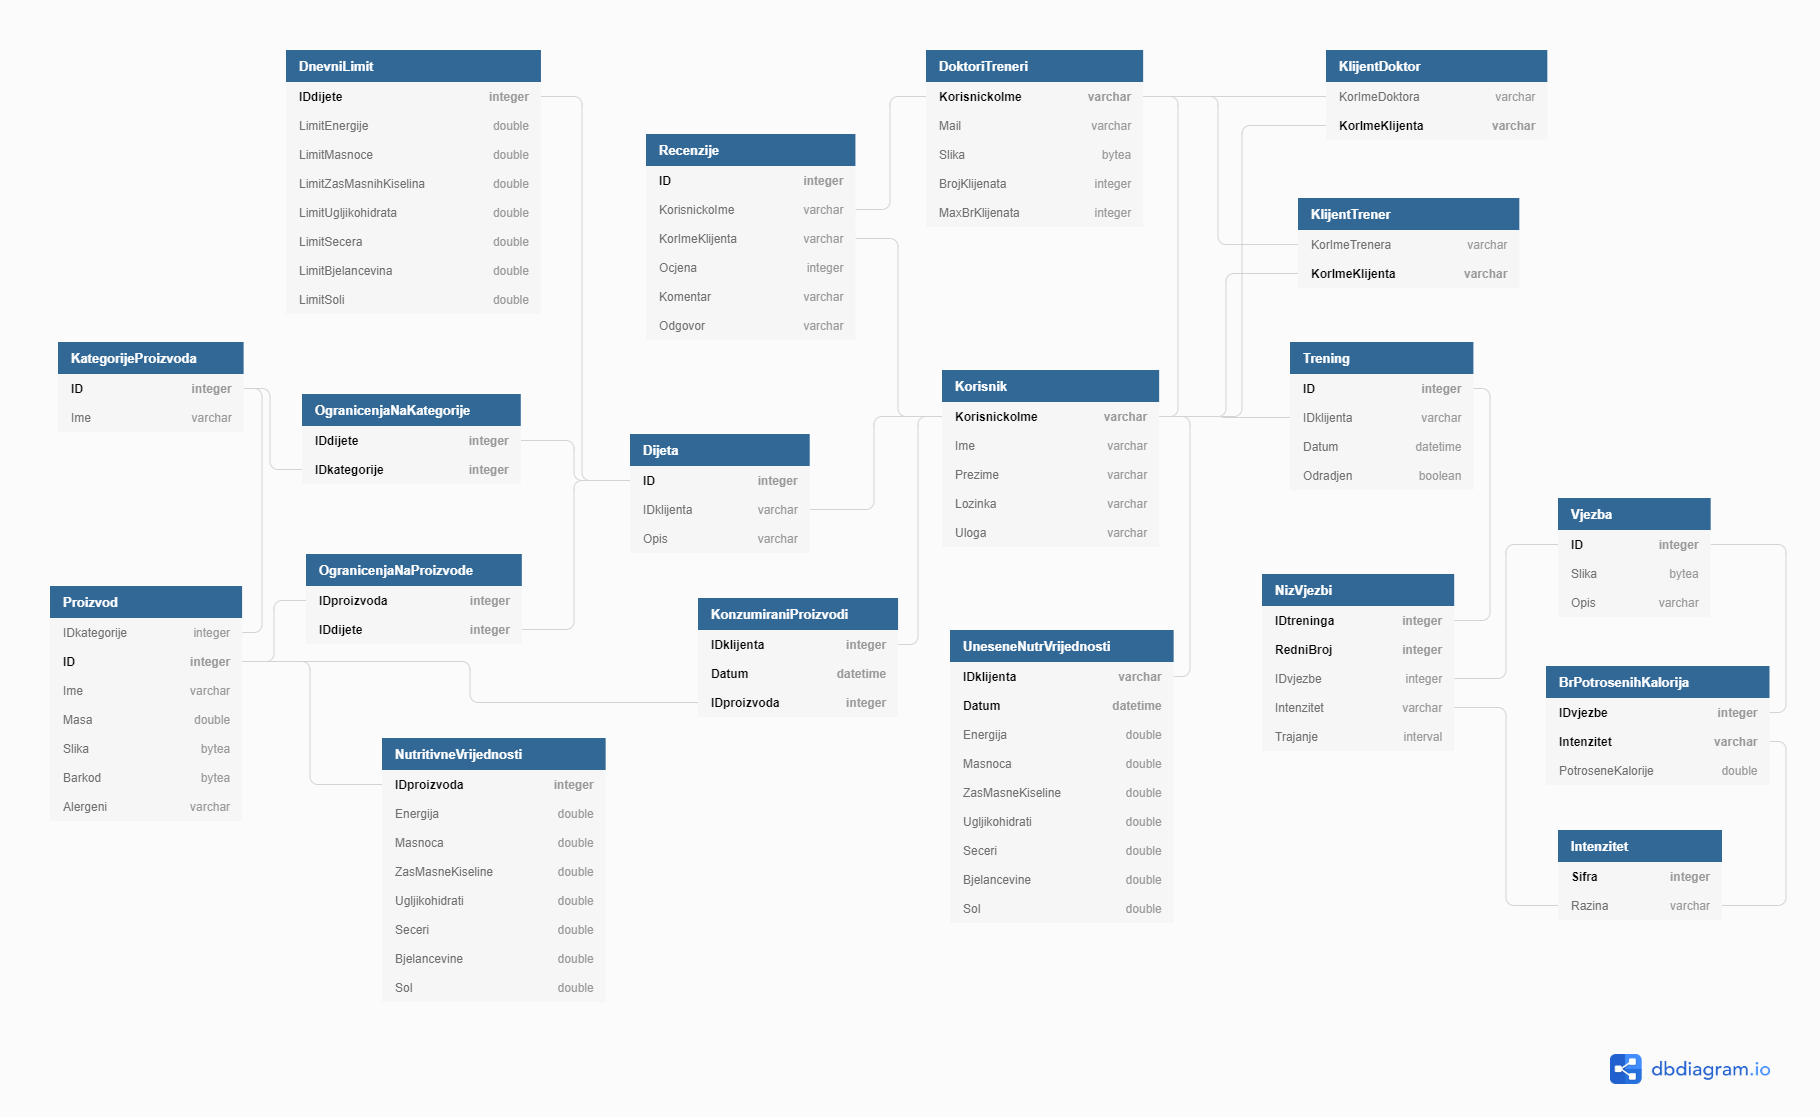
\includegraphics[width=\textwidth,height=\textheight,keepaspectratio]{slike/dijagramBaze.png}
					\centering
					\caption{Dijagram baze podataka}
					\label{fig:promjene}
				\end{figure}
			
			\eject
			
			
		\section{Dijagram razreda}
		
			Na slikama 4.1 i 4.2 su prikazani razredi koji pripadaju backend dijelu MVC
			arhitekture. Razredi prikazani na slici 4.1 nasljeđuju Controller razred. Metode implementirane u Controller razredima vracaju JSON datoteke s html status kodom. 
			
			\begin{figure}[H]
			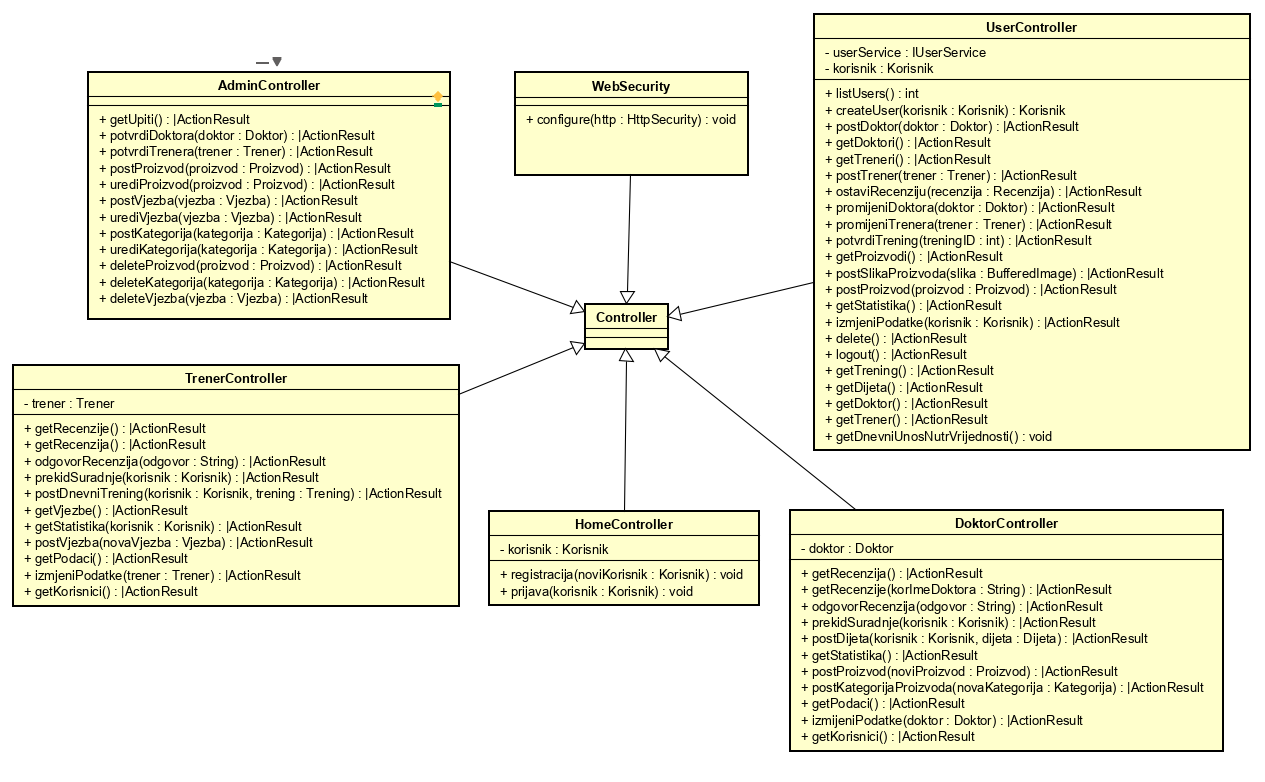
\includegraphics[scale=0.65]{slike/Controlleri.PNG}
			\centering
			\caption{Dijagram razreda - dio Controlleri}
			\label{fig:promjene}
			\end{figure}
			\eject
			Model razredi preslikavaju strukturu baze podataka u aplikaciji. Implementirane metode direktno komuniciraju s bazom podataka te vracaju tražene podatke. Razred Korisnik predstavlja registriranu osobu koja može stupiti u suradnju s doktorom i trenerom.Razred Trener predstavlja registrirnu osobu koju je dodatno potvrdio administrator.Njegova glavna uloga je osmišljavanje treninga, koji se sastoje od niza vježbi, svojim klijentima.Vježbe i treninzi su razredi sa svojim atributima.Razred Doktor perdstavlja registriranu osobu koju je također dodatno potvrdio administrator.Njegova glavna uloga je osmišljanje dijete koja se može sastojati od dnevnog limita pojedinih nutritivnih vrijednosti, specifičnih proizvoda ili kategorija proizvoda.Dijeta, Proizvod, Kategorija i Nutritivne Vrijednosti su razredi sa svojim atributima.Rezred Recenzija predstavlja osvrt klijenta na svog doktora ili trenera.
			
			Svi razredi realiziraju get i set metode za svoje atribute.
			\begin{figure}[H]
			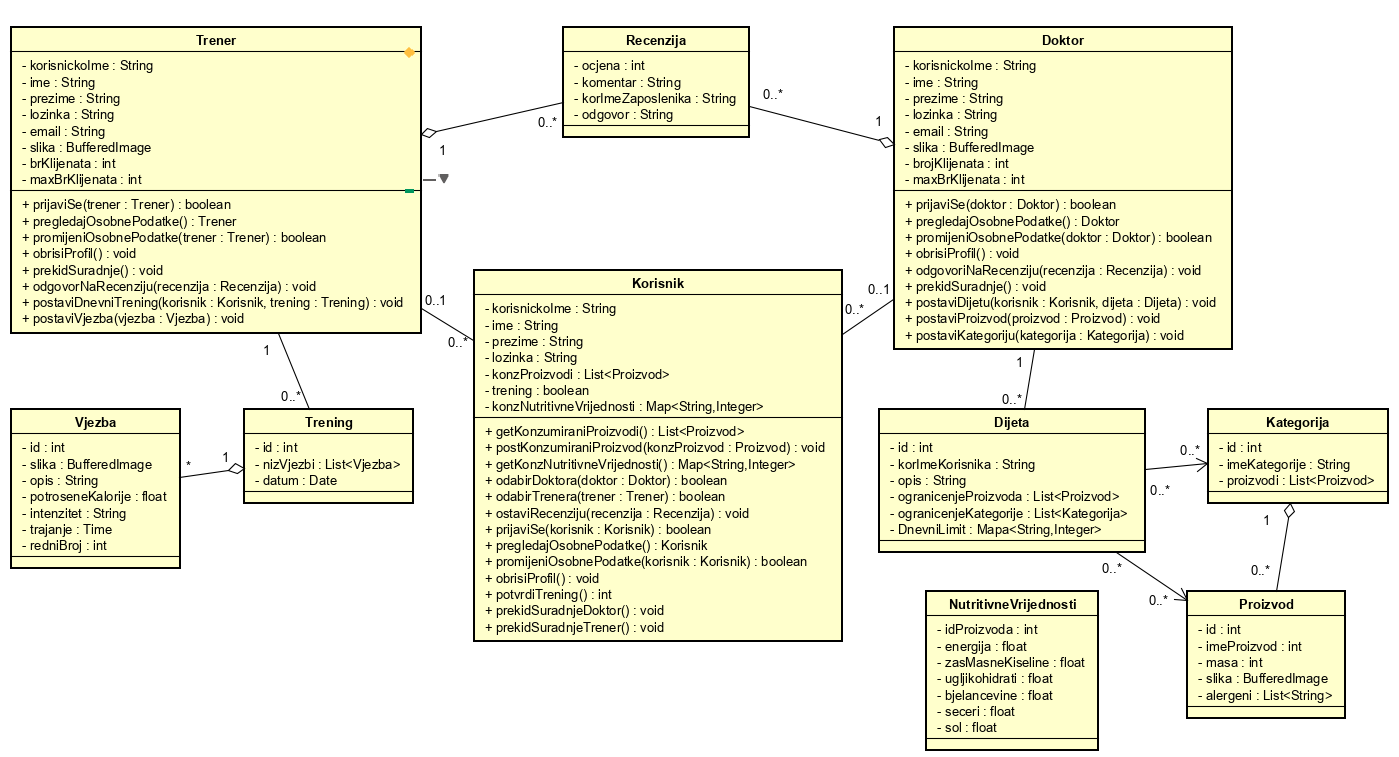
\includegraphics[scale=0.6]{slike/Modeli.PNG}
			\centering
			\caption{Dijagram razreda - dio Modeli}
			\label{fig:promjene}
			\end{figure}
			\eject
			
			\textbf{\textit{dio 2. revizije}}\\			
			
			\textit{Prilikom druge predaje projekta dijagram razreda i opisi moraju odgovarati stvarnom stanju implementacije}
			
			
			
			\eject
		
		\section{Dijagram stanja}
			
			
			\textbf{\textit{dio 2. revizije}}\\
			
			\textit{Potrebno je priložiti dijagram stanja i opisati ga. Dovoljan je jedan dijagram stanja koji prikazuje \textbf{značajan dio funkcionalnosti} sustava. Na primjer, stanja korisničkog sučelja i tijek korištenja neke ključne funkcionalnosti jesu značajan dio sustava, a registracija i prijava nisu. }
			
			
			\eject 
		
		\section{Dijagram aktivnosti}
			
			\textbf{\textit{dio 2. revizije}}\\
			
			 \textit{Potrebno je priložiti dijagram aktivnosti s pripadajućim opisom. Dijagram aktivnosti treba prikazivati značajan dio sustava.}
			
			\eject
		\section{Dijagram komponenti}
		
			\textbf{\textit{dio 2. revizije}}\\
		
			 \textit{Potrebno je priložiti dijagram komponenti s pripadajućim opisom. Dijagram komponenti treba prikazivati strukturu cijele aplikacije.}